\documentclass{beamer}
\usepackage{amsmath,amssymb,amsthm,array}
\usepackage{xltxtra}
\usepackage{multirow}
\usepackage{multicol}
\usepackage{algorithm}
\usepackage{algorithmic}
\usetheme{CambridgeUS}
\usecolortheme{seahorse}
\usefonttheme{serif}
\setmainfont[Mapping=TeX-text]{GFS Neohellenic}
\setbeamertemplate{navigation symbols}{}
\title{Attacks On Mixnets}
\author{Panagiotis Grontas}
\defbeamertemplate*{footline}{shadow theme}
{%
  \leavevmode%
  \hbox{\begin{beamercolorbox}[wd=.5\paperwidth,ht=2.5ex,dp=1.125ex,leftskip=.3cm plus1fil,rightskip=.3cm]{author in head/foot}%
    \usebeamerfont{author in head/foot}\insertframenumber\,/\,\inserttotalframenumber\hfill\insertshortauthor (\insertshortinstitute)
  \end{beamercolorbox}%
  \begin{beamercolorbox}[wd=.5\paperwidth,ht=2.5ex,dp=1.125ex,leftskip=.3cm,rightskip=.3cm plus1fil]{title in head/foot}%
    \usebeamerfont{title in head/foot}\insertshorttitle%
  \end{beamercolorbox}}%
  \vskip0pt%
}
\institute{$\mu\Pi\lambda\forall$  - CoReLab Crypto Group}

\setlength{\columnseprule}{0.4pt}
\begin{document}

\begin{frame}
\titlepage
\end{frame}

\begin{frame}{Overview}

\begin{block}{Attack Targets}
\begin{itemize}
\item \textbf{Privacy} Expose the messages of one or more senders
\item \textbf{Correctness} Alter the output of the mixnet
\item \textbf{Robustness} Bypass honest mix servers, so they cannot detect/defeat any cheating attempt
\end{itemize}
\end{block}

\begin{block}{Attack Options}
\begin{itemize}
\item Corrupt One Or More Senders
\item Corrupt One Or More Mix Servers
\item Corrupt Both
\item Exploit Protocol Weaknesses
\end{itemize}
\end{block}

\end{frame}


\section{Pfitzmann Attacks}

\begin{frame}{Related input attack}
\begin{center}
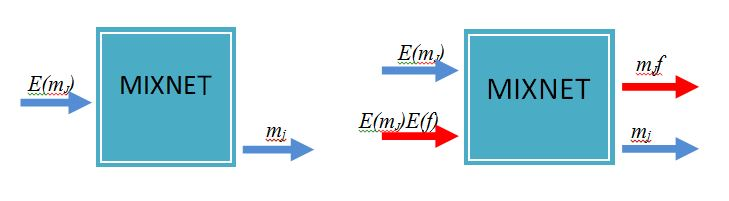
\includegraphics[scale=0.4]{PC.JPG}
\end{center}
\end{frame}

\begin{frame}[allowframebreaks]{Chaumian Mixnets}
\begin{itemize}
\item Active Attack 
\item Idea:Trace a message $m$ using RSA multiplicative homomorphism
\begin{center}
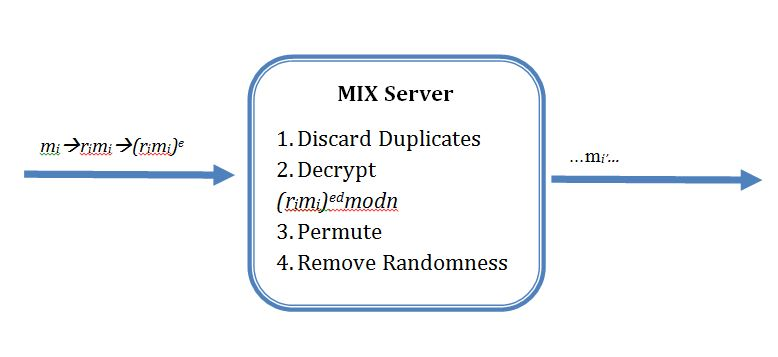
\includegraphics[scale=0.3]{chaumian.jpg}
\end{center}
\item Apply randomness of length $b$ to message of length $B$
\item Mixnet input: $\mathcal{E}(m) = (r \cdot 2^B + m)^e mod n$
\item Mixnet output: $m$
\end{itemize}
\begin{block}{The Attack}
\begin{small}
\begin{enumerate} 
\item Choose a small factor $f$
\item For the message $m$ to be tracked input to the mixnet the message 
$\mathcal{E}(m) \cdot \mathcal{E}(f) = (r \cdot 2^B + m)^e \cdot f^e mod n$
\item Mixnet operates as usual, considering input of the form: $(r^* \cdot 2^B + m^*)^e$
\item As a result: 
\begin{align*}
(r^* \cdot 2^B + m^*) = (r \cdot 2^B + m) \cdot f  \Rightarrow \\
(m^* - f \cdot m) \cdot 2^{-B} = (f \cdot r  -  r^*)
\end{align*}
\item Fact 1:$m^*, m \in$ mix output
\item Fact 2:$r,r^* \in \{0, \cdots, 2^b - 1\} \Rightarrow (f \cdot r  -  r^*) \in  \{2^{-b} + 1, \cdots, f \cdot (2^b - 1)\}$
\item For all output message pairs $(m,m^*)$ check for which $(m^* - f \cdot m)$ has a value in $\{2^{-b} + 1, \cdots, f \cdot (2^b - 1)\}$
\end{enumerate} 
\end{small}
\end{block}
\end{frame}

\begin{frame}[allowframebreaks]{Reencryption Mixnets}
\begin{block}{The Passive Attack}
\begin{itemize}
\item ElGamal is not semantically secure for any prime $p$
\item Only safe primes $p=2q+1$ must be used
\item Choose the generator from subgroup $\mathbb{Z}_q$
\end{itemize}
\end{block}

\begin{block}{The Active Attack - Decryption Mixnets}
\begin{itemize}
\item Track input $m_i$ for participant $P_i$:
\item Initial Encryption $c_{i0} = (g^R, m_i \cdot (y_1,\cdots,y_k)^R)$
\item Mix server j input: $c_{ij} = (g^{R'}, m_i \cdot (y_j,\cdots,y_k)^{R'}) = (t,u)$
\item For some random $x$ generate $c^{''}_{ij} = (t^x,u^x)=(g^{R'x}, m_{i}^{x} \cdot (y_j,\cdots,y_k)^{R'x})$
\item Output will contain both $m_{i}^{x},m_{i}$
\item Raise all output messages to the $x$ and check for duplicates.
\end{itemize}
\end{block}

\begin{block}{Remarks}
\begin{itemize}
\item If there is a check on number of input items a colluding participant's message must be omitted
\item Solution: Redundancy in messages in order to detect the attack
\begin{itemize}
\item Increases Ciphertext Size
\item Does not work if the last mix server is corrupt, since it can replace the $m_{i}^{x}$ with a correct looking message after the message correlation
\end{itemize} 
\item Detection: DDH Assumption
\end{itemize}
\end{block}
\end{frame}

\section{Attacks on Sako-Killian}

\begin{frame}[allowframebreaks]{A single honest mix server can be overriden}
\begin{block}{Attack on Privacy}
\begin{itemize}
\item Break voter privacy even when there is only one honest mix server $M_j$
\item No colluding voters are needed
\end{itemize}
\end{block}
\begin{itemize}
\item Each mix server
\begin{itemize}
\item Proves that can decrypt
\item Reencrypts - Proves Reencryption
\item Shuffles - Proves Shuffle
\end{itemize}
\item The attack happens before $M_j$ performs the shuffle
\item The first $j-1$ corrupt mix servers trace the message to be revealed
\item The last $k-j$ servers reveal the message
\end{itemize}
\framebreak

\textbf{Details}

\begin{itemize}
\item Voter Alice sends to $M_1$ her input m as
\[
(G_1,M_1) = (g^{r_0},m \cdot (\prod_{t=1}^{k} y_t)^{r_0})
\]

\item Honest Mix Server receives: 
\[
 (G_j,M_j) = (g^{r_0+R},m \cdot (\prod_{t=j}^{k} y_t)^{r_0+R}) \text{ where } R=\sum_{t=1}^{j-1} r_t
\]

\item Honest Mix Server follows the protocols and reveals in order to prove that he can partially decrypt correctly.
\[
H_j = G_{j}^{x_j} = (g^{r_0+R})^{x_j} 
\]


\item The rest of the corrupted servers contribute their private keys $x_j$ and compute:
\[
\frac{M_j}{H_j \cdot \prod_{t=j+1}^{k} G_{j}^{x_t}} = \frac {m \cdot (\prod_{t=j}^{k} y_t)^{r_0+R}} {(g^{r_0+R})^{x_j} \cdot  (g^{r_0+R})^{\sum_{t=j+1}^{k} x_t}} = m
\]
\end{itemize}

\begin{block}{A simple countermeasure}
First shuffle then reencrypt
\end{block}

\end{frame}

\section{Wikstr\"om Attacks On Optimistic Mixing}

\begin{frame}[allowframebreaks]{Break privacy when all servers are honest}
\begin{block}{Requirements}
Attacker can send 2 messages to the mixnet (by corrupting two voters)
\end{block}

\begin{itemize}
\item Target user Alice submits message $m$ to mixnet
\item $m \rightarrow_{E_1}  \rightarrow (\mu_1,\mu_2) \rightarrow_{H} \rightarrow (\mu_1,\mu_2,w) \rightarrow_{E_2} $
\item Randomly select $\gamma,\delta$
\item Calculate 
	  \small \[ \mu_1^\delta,\mu_2^\delta,w_\delta=H(\mu_1^\delta,\mu_2^\delta) \] \normalsize
	  and 
	  \small \[ \mu_1^\gamma,\mu_2^\gamma,w_\gamma=H(\mu_1^\gamma,\mu_2^\gamma) \] \normalsize
\item Calculate and submit 
	  \small \[ E(\mu_1^\delta),E(\mu_2^\delta),E(w_\delta)  \text{ and } E(\mu_1^\gamma),E(\mu_2^\gamma),E(w_\gamma) \] \normalsize
\item Mixnet operates as usual and since all mix servers are honest removes both layers of encryption!
\item Attacker raises outputs to $\frac{\delta}{\gamma}$ \\
\tiny
$ output \rightarrow_{D_1}
 \left[ \begin{array}{c} (u_1,v_1,w_1) \\ \cdots \\ \mu_1^\delta,\mu_2^\delta,w_\delta \\ \cdots \\ \mu_1,\mu_2,w \\ \cdots \\  \mu_1^\gamma,\mu_2^\gamma,w_\gamma \\ \cdots \\ (u_N,v_N,w_N) \end{array} \right] \rightarrow_{D_2 \text{to produce} L_k}
\left[ \begin{array}{c} m_1 \\ \cdots \\ m_x = m^\delta \\ \cdots\\ m \\ \cdots\\  \\ m_y =  m^\gamma \\ \cdots \\ m_N \end{array} \right] \rightarrow_{ \text{ raise to } \frac{\delta}{\gamma} \text{to produce } L^{'}_{k}}
\left[ \begin{array}{c} m_1^{\frac{\delta}{\gamma}} \\ \cdots \\ m_x^{\frac{\delta}{\gamma}} \\ \cdots \\ m^{\frac{\delta}{\gamma}} \\ \cdots \\ m_y^{\frac{\delta}{\gamma}} = m_x \\ \cdots \\ m_N^{\frac{\delta}{\gamma}} \end{array} \right] 
$
\end{itemize}
\framebreak
\normalsize

\begin{columns}[onlytextwidth]

\begin{column}{0.5\textwidth}
\begin{itemize}
\item Calculate $m_{y}^{\frac{1}{\gamma}} = m$
\item Find index $l$ of message m
\item Find ciphertext of index $l$
\item Search initial encryption for ciphertext corresponding to l
\item Alice is revealed
\item Remark: Can be generalised to break the privacy of $s$ senders
\end{itemize}
\end{column}


\begin{column}{0.5\textwidth}
\textbf{Exploits}
\begin{itemize}
\item Proof of ciphertext knowledge and not of message
\item Same keys for both layers of encryption
\end{itemize}
\end{column}

\end{columns}

\end{frame}

\begin{frame}[allowframebreaks]{Different Keys and Corrupt Mix Server}
\begin{block}{Requirements}
\begin{itemize}
\item Inner Encryption (Initial): $E_{in}$
\item Outer Encryption (On triples): $E_{out}$
\item 2 mix sessions with the same keys (unclear protocol assumption)
\item First mix server is corrupted and is identified in the first mix session
\end{itemize}
\end{block}
\begin{block}{First Mix Session}
\begin{itemize}
\item Target user Alice with message $m$ and user Bob with message $m'$
\item Corrupted mix server swaps encryption of hashes 
\[ m \rightarrow E_{in} \rightarrow (u,v) \rightarrow H \rightarrow w \rightarrow E_{out} \rightarrow [E_{out}(u),E_{out}(v),E_{out}(w')]=\alpha \]
and
\[ m' \rightarrow E_{in} \rightarrow (u',v') \rightarrow H \rightarrow w' \rightarrow E_{out} \rightarrow [E_{out}(u'),E_{out}(v'),E_{out}(w)]=\alpha' \]
\item Protocol proceeds as usual
\item Output contains two invalid tuples $(u,v,w')$ and $(u',v',w)$
\item Back-Tracing reveals first mix server as cheater \textbf{BUT}
\item Links Alice to $(u,v)$ and Bob to $(u',v')$
\end{itemize}
\end{block}

\begin{block}{Second Mix Session - Decryption Oracle}
\begin{itemize}
\item Relation attack on Alice's ciphertext $(u,v)$
\item Randomly select $\gamma,\delta$
and Calculate 
	  \small \[ u^\delta,v^\delta,w_\delta=H(u^\delta,v^\delta) \] \normalsize
	  and 
	  \small \[ u^\gamma,v^\gamma,w_\gamma=H(u^\gamma,v^\gamma) \] \normalsize
\item Calculate and submit 
	  \small \[ E_{out}(u^\delta),E_{out}(v^\delta),E_{out}(w_\delta)  \text{ and } E_{out}(u^\gamma),E_{out}(v^\gamma),E_{out}(w_\gamma) \] \normalsize
\item Mixnet operates as usual and since all mix servers are honest (now) removes both layers of encryption!
\item Attacker raises outputs to $\frac{\delta}{\gamma}$ and correlates messages as before
\end{itemize}
\textbf{Exploit}: Proof of knowledge of ciphertext and not of message!
\end{block}
\end{frame}

\begin{frame}[allowframebreaks]{Attack On Privacy without corrupted users}
\begin{block}{Requirements}

\begin{itemize}
\item Honest Senders
\item Last Mix Server $M_k$ is corrupted
\item \textbf{Objective:} Break privacy of all users
\end{itemize}

\end{block}

\begin{block}{Actions of $M_k$}
\begin{enumerate}
\item Generate the tuple $(a',b', \cdots, f') = (\frac{a_{k-1}}{a_0},\frac{b_{k-1}}{b_0}, \cdots, \frac{f_{k-1}}{f_0})$
		where $a_j = \prod_{i=1}^N a_{ji}$ the product of the first components of the $N$ inputs of $M_j$
\item Generate the tuple $\alpha_1 = (a' \cdot a_{01}, \cdots, f' \cdot f_{01}) $
\item Generate the list $L'_{k-1}$ by retrieving $L_0$, the input list to the mixnet, and replacing the first message with $\alpha_1$
\item Instead of processing the normal input list $L_{k-1}$  process the list $L'_{k-1}$.
\item Mixnet output is a permutation and reencryption of $L'_{k-1}$, essentially of $L_0$
\item If $M_k$ isn't caught then after decryption, privacy is broken!
\end{enumerate}
\end{block}

\begin{block}{Corrupted Server passes verification}
\begin{itemize}
\item Proof of correct reencryption
\begin{itemize}
\item The modification to the input list is \textit{invisible}
\[ \ a'_{k-1}  = a'a_{01} \cdot \prod_{i=2}^N a_{0i} =  a' \cdot \prod_{i=1}^N a_{0i} = a' \cdot a_0 = \frac{a_{k-1}}{a_0} \cdot a_0 =  \ a_{k-1}  \]
\item Subsequently $M_k$ behaves honestly
\end{itemize}
\item Invalid Triples Investigation 
\item $M_k$ cannot correlate the real $L_{k-1}$ with $L_k$ but it is not necessary as:
\begin{itemize}
\item All users are honest
\item All mix servers except $M_k$ are honest
\item $M_k$ does not corrupt inner triples
\item There are no invalid triples
\end{itemize}
\end{itemize}
\end{block}
\end{frame}

\begin{frame}[allowframebreaks]{Two corrupted mix servers}
\begin{block}{Requirements}
\begin{itemize}
\item Honest Senders
\item First $M_1$ and Last  $M_k$ Mix Server is corrupted
\item \textbf{Objective:} Break privacy of a particular user
\end{itemize}
\end{block} 

\begin{block}{Main idea}
\begin{itemize}
\item Let $P,Q$ the primes in the initialisation of the El Gamal Cryptosystem
\item All ciphertexts should be in $G_Q$
\item If no check is made, we can use elements in $\mathbb{Z}_P^* - G_Q$ to 'tag' messages and break privacy
\end{itemize}
\end{block}

\begin{block}{The attack}
\begin{itemize}
\item Corrupt mix server $M_1$ and select $\gamma \in_R \mathbb{Z}_P^* - G_Q$
\item Compute $ \alpha_1' = (\gamma \cdot a_{01}, \cdots,  f_{01}) $ where $\alpha_1$ is the message of Alice (target) and $ \alpha_2' = (\gamma^{-1} \cdot a_{02}, \cdots,  f_{02}) $ where $\alpha_2$ is the message of another user Bob.
\item Replace $ \alpha_1 $ with $ \alpha_1' $ and $ \alpha_2 $ with $ \alpha_2' $ and proceed as usual
\item Corrupt mix server $M_{k-1}$ receives input $L_{k-1}$ and processes it as usual
\item Output would be $L_k = \{ \beta_i \}_{i=1}^{N} =  \{ (\cdot a_{ki}, \cdots,  f_{ki}) \}_{i=1}^{N} $
\item Search for $l, l'$ st: $a_{kl}^Q = \gamma ^ Q, \, a_{kl'}^{Q}= \gamma ^ {-Q} $
\item Replace $ \beta_l $ with $ (\gamma^{-1}a_{kl}, \cdots, f_{kl})   $ and $ \beta_{l'} $ with $ (\gamma^a_{kl'}, \cdots, f_{kl'})  $
\item Output the result. Decryption takes place. Alice's message is $m_l$
\end{itemize}
\end{block}

\begin{block}{Justification}
\begin{itemize}
\item Attack works because: $\forall b \in G_Q : b^Q = 1$. As a result $a_{kl}^Q = \gamma ^ Q (g^r a_{01})^Q = \gamma ^ Q$
\item Attack passes validations since only the a-component of the tuple is changed and  
\item Products are left unchanged as:
\[ \ a_{1}  = \gamma a_{01} \gamma^{-1} a_{02} \prod_{i=3}^N a_{0i} = \prod_{i=1}^N a_{0i} = \ a_{1} \] and
\[ \ a_{k}  = \gamma a_{kl'} \gamma^{-1} a_{kl} \prod_{i \neq l,l'}^N a_{0i} = \prod_{i=1}^N a_{ki} = \ a_{k} \]
\end{itemize}
\end{block}

\end{frame}

\begin{frame}[allowframebreaks]{Delayed Effect Attack}
\begin{block}{Requirements}
\begin{itemize}
\item Corrupted First Mix Server
\item Even Number Of Corrupted Senders
\end{itemize}
\end{block}

\begin{block}{Main idea}
The adversary can cancel out the cheating based on an event after the vote casting phase.
\textbf{Example:} Double elections. The adversary might inject votes in the second election, but depending on the first outcome he might cancel them out.
\end{block}

\begin{itemize}
\item Casted votes are $ x_i = (a_i,b_i,c_i,d_i,e_i,f_i) = (E(u_i),E(v_i),E(w_i)), i=1,\cdots,N $
\item Select $z \in G_Q$ and two voters $k,l$ and compute  $x_k' = (a_i,b_i,c_i,zd_i,e_i,f_i) $ and $x_l' = (a_i,b_i,c_i,z^{-1}d_i,e_i,f_i) $
\item Product is maintained
\item Replace $x_k, x_l$
\item $M_1$ Might choose to correct them or not
\end{itemize}

\end{frame}


\section{Wikstr\"om attacks on RPC}

\begin{frame}[allowframebreaks]{Pfitzmann Attacks work with probability $\frac{1}{2}$}
\begin{block}{Requirements}
\begin{itemize}
\item Corrupted Mix Servers: First
\item Voters: One / None
\end{itemize}
\end{block}

\begin{block}{Trace a single message}
\begin{itemize}
\item Submitted ciphertext is $c$
\item Corrupted mix server chooses an integer $\delta$
\item Replace an output by $c^\delta$
\item This is not detected during verification with probability $\frac{1}{2}$
\item Search the output for messages $m, m*$ st $m*=m^\delta$
\item Ciphertext $c$ was encryption of $m$
\end{itemize}
\end{block}
\begin{block}{Trace multiple messages}
\begin{itemize}
\item Submitted ciphertexts is $\{c_i\}_{i=1}^s$
\item Corrupted mix server chooses integers$\{\delta_i\}_{i=1}^s$
\item Replace an output by $\prod_{i=1}^s c_i^{\delta_i}$
\item This is not detected during verification with probability $\frac{1}{2}$
\item Search the output for messages $\{m_i\}_{i=1}^s, m*$ st $m*=\prod_{i=1}^s m_i^{\delta_i}$
\item Correspondence for $m_i$ is revealed
\end{itemize}
\end{block}
\end{frame}

\begin{frame}[allowframebreaks]{On duplicate removal}

\begin{block}{Requirements}
\begin{itemize}
\item Chaumian Mixnet
\item Corrupted Mix Servers: First and Last
\item Corrupted Voters:   $\frac{s(s+1)}{2}$
\end{itemize}
\end{block}

\begin{block}{Actions of first mix server}
\begin{itemize}
\item Target ciphertexts  $\{c_i\}_{i=1}^s$
\item First mix server removes first layer of encryption
\item For $c_{i1}$ make $i$ independent encryptions using his public key
\item Replace $\frac{s(s+1)}{2}$ ciphertexts with the duplicate encryptions
\item These encryptions replace the original messages
\end{itemize}
\end{block}

\begin{block}{Actions of last mix server}
\begin{itemize}
\item Input contains duplicate items ($i+1$ for ciphetext $i$)
\item Decrypt using public key as always
\item Identify correspondence based on the number of duplicates
\item $s+\frac{s(s+1)}{2} \leq N $
\item The privacy of $O(\sqrt{N})$ voters can be broken
\end{itemize}
\end{block}

\begin{block}{A simple countermeasure}
Remove duplicates everywhere
\end{block}

\end{frame}

\begin{frame}[allowframebreaks]{Commitments must be valid permutations}

\begin{block}{Requirements}
\begin{itemize}
\item Reencryption Mixnet
\item Corrupted Mix Servers: First and Second (operated by a single entity)
\item Corrupted Voters: 2
\end{itemize}
\textbf{Target:}Break Privacy Undetected
\end{block}


\begin{block}{Initialisation}
\begin{itemize}
\item Submitted ciphertexts is $\{c_i\}_{i=1}^s$
\item Attacker chooses integers$\{\delta_i\}_{i=1}^s$
\item Calculate $c=\prod_{i=1}^s c_i^{\delta_i}$
\item Corrupted senders posts 2 messages that are reencryption of each other $c_{i_1,0},c_{i_2,0}$
\end{itemize}
\end{block}

\begin{block}{$M_1$}
\begin{itemize}
\item Keep track of corrupted messages permutations
\item Keep track of reencryption randomness
\end{itemize}
\end{block}

\begin{block}{$M_2$}
\begin{itemize}
\item Commit $c_{i_1},c_{i_2}$ to same output $\pi_2(i_1)$.
\item Replace output $\pi_2(i_2)$ with $c$
\end{itemize}
\end{block}

\begin{center}
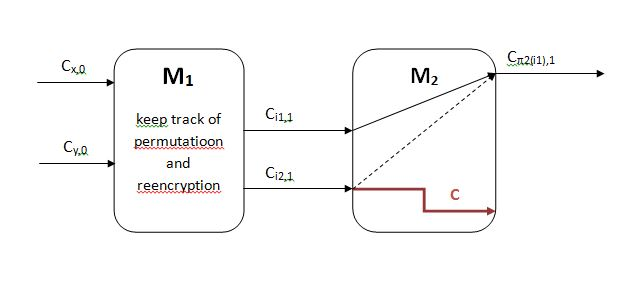
\includegraphics[scale=0.4]{rpc.jpg}
\end{center}

\begin{block}{After mixing}
\begin{itemize}
\item Search the output for messages $\{m_i\}_{i=1}^s, m*$ st $m*=\prod_{i=1}^s m_i^{\delta_i}$
\item Correspondence for $m_i$ is revealed without detection
\end{itemize}
\end{block}

\begin{block}{Attack goes undetected}
\begin{itemize}
\item Both commitments verify since $c_{i_1},c_{i_2}$ are reencryptions of the same message
\item $M_2$ can provide the randomness to prove it
\end{itemize}
\end{block}

\begin{block}{Generalisation}
\begin{itemize}
\item $r+1$ reeencryptions of a message 
\item $r+1$ false commitments
\item $r \cdot s$ messages
\end{itemize}
\end{block}

\begin{block}{Rig an election undetected}
\begin{itemize}
\item Corrupt the first mix server and the first sender
\item First sender sends m as plaintext $c_{10} = Enc(m)$
\item Replace all the ciphertexts with $c_{10}$
\item Corrupted mix server commits all outputs to 1
\item Corrupted Mix Server can pass verification
\item \textbf{Realistic scenario:} Replace the actual outputs with the distribution of votes that he likes
\end{itemize}
\end{block}
 

\begin{columns}[onlytextwidth]

\begin{column}{0.6\textwidth}
Unopened Commitments
\begin{itemize}
\item Unopened commitments might not be consistent with a permutation
\item Replace a message sent by an honest sender with a cheating message
\item Commit to the same output
\item Detection: Open both commitments
\item Detection probability $\frac{1}{4}$
\item Repeat $t$ times with success probability $(\frac{3}{4})^t$
\end{itemize}
\end{column}

\begin{column}{0.4\textwidth}
\begin{center}
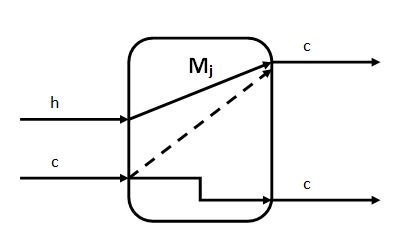
\includegraphics[scale=0.3]{rpc2.jpg}
\end{center}
\end{column}

\end{columns}

\end{frame}



\section{Attacks On The Scytl Mixnet}

\begin{frame}[allowframebreaks]{The Scytl Mixnet \cite{SCYTL10}}
\begin{itemize}
\item Proposed by Puiggali and Castello in 2010
\item Commercial Use from Scytl
\item Part of the Norwegian 2011 municipal elections
\item Operation based on
\begin{itemize}
	\item Randomised Partial Checking (RPC)
	\item Almost Entirely Correct Mixing
	\item Optimised Mixing
\end{itemize}
\item Reencryption based mixnet
\item Main Idea
\begin{itemize}
\item Verification occurs after operation and before decryption
\item Inputs and outputs are split into groups
\item Group membership is revealed for all votes
\item Verification by comparing $\prod inputs$ with $\prod outputs$ for each group
\item Verification is done in Zero-Knowledge
\end{itemize}
\end{itemize}
\begin{block}{Verification}
\begin{itemize}
\item Verifier groups encrypted input
\item For each output the prover reveals the input group
\item Verifier calculates:
\begin{itemize}
\item \textbf{Input Integrity Proof:} Products per group of input votes
\item \textbf{Output Integrity Proof:} Products per input group of output proofs
\end{itemize}
\item ZK Proof that Output Integrity Proof is reencryption of Input Integrity Proof
\item Remarks
\begin{itemize}
\item Group size $l$ is constant
\item First grouping is random
\item Regrouping for $M_j$
\begin{itemize}
\item Sort outputs of $M_{j-1}$ by group index
\item Input group $\#1$ Receive \textit{first} item of each output group
\item Input group $\#2$ Receive \textit{second} item of each output group ...
\end{itemize}
\end{itemize}
\end{itemize}
\end{block}
\begin{center}
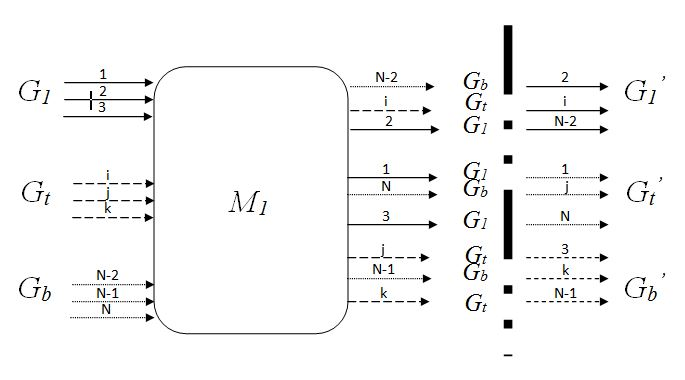
\includegraphics[scale=0.4]{scytl1.jpg}
\end{center}
\end{frame}

\begin{frame}{Basic Pfitzmann Attack}
\begin{itemize}
\item \textbf{Target:} privacy of $s$ voters with inputs $c_1,...,c_s$
\item \textbf{Requirements}: Corrupt 2 voters with inputs $c_{01},c_{02}$ and the first mix server
\item Select $s$ random exponents $\delta_1, ..., \delta_s$
\item Calculate $u_1=\prod_{i=1}^s c_i^{\delta_i}$ and $u_2 = \frac{c_{01} \cdot c_{02}}{u_1}$
\item Replace $c_{01},c_{02}$ with $u_1,u_2$
\item \textbf{Remark:} Product is preserved: $c_{01} \cdot c_{02} = u_1 \cdot u_2$
\item In order to pass verifcation $u_1,u_2$ must belong to the same block
\item \textbf{Success Probability:} $\frac{1}{b}$
\item After decryption, search $s+1$ messages such that $ m = \prod_{i=1}^s m_i^{\delta_i}$
\end{itemize}
\end{frame}

\begin{frame}[allowframebreaks]{Undetected Pfitzmann Attack}
\begin{itemize}
\item Target privacy of $s$ voters
\item 1 corrupted mix server
\item $B$ corrupted voters
\item The corrupted messages are reencryptions of each other
\item The corrupted mix server can handle them without affecting the verification process 
\end{itemize}
\begin{block}{The birthday paradox}
Pick $s$ elements of a multiset with $b$ elements. \\
Collision Probability $P(s,b) \geq 1 - e ^ \frac{-s^2}{2 \cdot b}$
\end{block}
\begin{itemize}
\item Very high probability of success with few corrupted voters
\item For $B=3 \cdot \sqrt{b}$ corrupted voters $98\%$ chance of success.

\end{itemize}

\framebreak

\begin{itemize}

\item $B$ corrupted messages
\item $u_1, u_2$ the 'malicious messages', $u_1=\prod_{i=1}^s c_i^{\delta_i}$ and $u_2 = \frac{c_{01} \cdot c_{02}}{u_1}$
\item $u_1, u_2$ must end up in the same input block
\item Say that $u_1, u_2$ exit the mix server at positions $e_1, e_2$
\item Let $i_1, i_2$ two corrupted messages that are indeed in the same input group
\item Say that $i_1, i_2$ exit at positions $x_1, x_2$
\item The corrupted mix server can swap u's with the i's to put them in the same block

\framebreak

\begin{center}
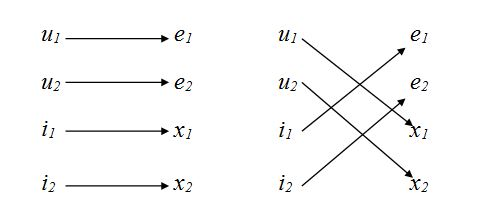
\includegraphics[scale=0.4]{scytl2.jpg}
\end{center}
\item Swapping can go undetected wvhp
\item Explanation
\begin{itemize}
\item The corrupted mix server must prove that $x_1 \cdot x_2 = ReEnc (i_1 \cdot i_2) $
\item But $ReEnc (i_1 \cdot i_2)= ReEnc (c_{01} \cdot c_{02}) = ReEnc (u_1 \cdot u_2)$
\item And of course by hushing up the replacement the other 'processing' can be proved as well
$e_1 = ReEnc(u_1) = ReEnc(i_1)$ and $e_2 = ReEnc(u_2) = ReEnc(i_2)$
\end{itemize}

\item \textit{Probability of success = Probability 2 corrupted messages end up in the same block}

\end{itemize}

\end{frame}

\begin{frame}[allowframebreaks]{Attack On Correctness}
\begin{block}{Overview}
\begin{itemize}
\item 1 corrupted mix server
\item $l \geq b$
\item \textbf{Target}: Replace $R=\frac{1}{3}\sqrt{b}-1$ votes without detection
\end{itemize}
\end{block}
\begin{itemize}
\item Corrupted mix server $M_j$ replaces first R+1 votes
\item The first corrupted votes $c_{j-1,1} \cdots c_{j-1,R}$ get replaced by 'malicious' messages $u_1, \cdots u_R$
\item In order to maintain the product the vote $c_{j-1,R+1}$ gets replaced by $\frac {\prod_{i=1}^{R+1} c_{j-1,i}} {\prod_{i=1}^R u_j}$

\framebreak

\item The replaced list $L'_{j-1}$ gets reencrypted and shuffled.
\item Probability that 2 integers in $\{1,R+1\} $are in the same block is $0.05$
\item With very high probability all such integers are in different blocks
\item By way of output partitioning all end up in the same output, with very highy probability. 
\item The proof is valid both for $L_{j-1}$ and $L'_{j-1}$.
\end{itemize}
\end{frame}


\begin{frame}[allowframebreaks]{References}
\begin{small}
\bibliographystyle{alpha}
\bibliography{attackref}
\end{small}
\nocite{*}
\end{frame}

 
\end{document}
